\subsection{Detectores de flancos}
\label{edgeDetectors}

Para la interfase del diseño con los pulsadores diseñamos dos detectores de flancos, uno estándar y otro antirrebotes, de forma que llegase un sólo pulso a los demás bloques del sistema por cada pulsación del jugador.

En el diseño final sólo hemos añadido el detector de flancos con antirrebote, debido a su mejor respuesta ante la entrada oscilante de los pulsadores reales.

\subsubsection{Detector de flancos estándar (edgeDetector)}
\label{edgeDetectorStd}
El detector de flancos estándar es un circuito muy simple. Se tienen dos biestables, uno almacenando el estado actual de la señal de entrada, y el otro almacenando el estado de la señal en el tiempo t-1.

Estas dos señales se comparan, y si hay un nivel alto en el estado actual, pero no en el anterior, entonces ha llegado un flanco, y el detector emite un pulso a la salida.


\subsubsection{Detector de flancos con antirrebote (edgeDetectorDebounce)}
\label{edgeDetectorDebounce}

\begin{figure}[H]
	\centering
	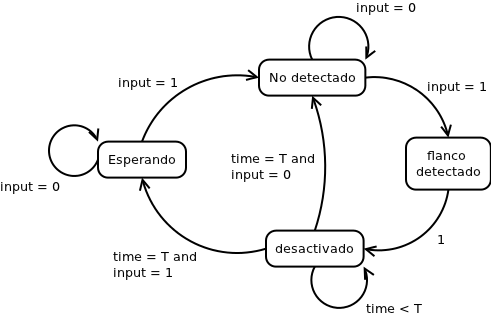
\includegraphics[width=0.5\textwidth]{edgeDetectorDebounceFSM.png}
	\caption{Máquina de estados}\label{fig:edgeDetectorDebounceFSM}
\end{figure}

El detector de flancos con antirrebote es un detector de flancos estándar al que se le ha añadido un temporizador que lo desactiva durante un cierto periodo de tiempo tras detectar un flanco, para evitar las oscilaciones producidas por los rebotes de los pulsadores.

Su diseño está basado en una máquina de estados simple (figura \ref{fig:edgeDetectorDebounceFSM}) que consta de cuatro estados: ``no detectado'', ``flanco detectado'', ``desactivado'' y ``esperando''. La máquina empieza en el estado ``no detectado'', y permanece en él mientras la entrada valga 0. Cuando recibe un 1, pasa al estado ``flanco detectado'', y la salida se pone a 1 hasta el siguiente flanco de reloj, en el cual pasa al estado
``desactivado'', poniendo la salida a 0. Mientras la máquina se encuentra en este estado, un temporizador cuenta el tiempo transcurrido, y bloquea el paso al estado siguiente. Cuando el tiempo deseado, en nuestro caso 100 ms,  ha transcurrido, la máquina de estados pasará al estado ``no detectado'' si la entrada es 0 o a ``esperando' si es 1. La máquina pasará entonces al estado de ``no detectado'' cuando reciba un 0 lógico.